%\documentclass[handout]{beamer}
\documentclass{beamer}

%-----------------------------
%           PACKAGES

\usepackage[T1]{fontenc}
\usepackage[utf8]{inputenc}
\usepackage{eulervm}
\usepackage[scaled]{helvet}
\usepackage{graphicx}
\usepackage{amsmath,amsfonts,amssymb}
\usepackage{tikz}
\usepackage{multicol}

\usetheme{Warsaw}
%\usetheme{Antibes}
%\usetheme{Montpellier}
%\usetheme{JuanLesPins}
%\usetheme{Goettingen}
\usefonttheme[onlymath]{serif}
\usecolortheme{Ben}
%\usecolortheme{fly}


\makeatletter
\def\insertsectionnavigation#1{%
  \hbox to #1{\vbox{{\usebeamerfont{section in head/foot}%
     \usebeamercolor[fg]{section in head/foot}%
     \def\slideentry##1##2##3##4##5##6{}%
     \def\sectionentry##1##2##3##4##5{%
       \ifnum##5=\c@part%
       \def\insertsectionhead{##2\hskip1em}%
       \def\insertsectionheadnumber{##1}%
       \def\insertpartheadnumber{##5}%
         \hyperlink{Navigation##3}{%
             \ifnum\c@section=##1%
               {\usebeamertemplate{section in head/foot}}%
             \else%
               {\usebeamertemplate{section in head/foot shaded}}%
             \fi%
         }\par
       \fi}%
       \parbox[c][0cm][c]{.5\paperwidth}{%
       \begin{multicols}{2}
       \dohead
       \end{multicols}}\space}
     }%
  \hfil}%
}

\def\insertsubsectionnavigation#1{%
  \hbox to #1{%
    \vbox{{%
      \usebeamerfont{subsection in head/foot}\usebeamercolor[fg]{subsection in head/foot}%
      \vskip0.5625ex%
      \beamer@currentsubsection=0%
      \def\sectionentry##1##2##3##4##5{}%
      \def\slideentry##1##2##3##4##5##6{\ifnum##6=\c@part\ifnum##1=\c@section%
        \ifnum##2>\beamer@currentsubsection%
        \beamer@currentsubsection=##2%
        \def\insertsubsectionhead{##5}%
        \def\insertsectionheadnumber{##1}%
        \def\insertsubsectionheadnumber{##2}%
        \def\insertpartheadnumber{##6}%
        \beamer@link(##4){%
              \ifnum\c@subsection=##2%
                {\usebeamertemplate{subsection in head/foot}}%
              \else%
                {\usebeamertemplate{subsection in head/foot shaded}}%
              \fi\hfill}\par
        \fi\fi\fi}%
       \hspace*{0.5em}\parbox[c][0cm][c]{\dimexpr.5\paperwidth-1em\relax}{%
       \begin{multicols}{2}
       \dohead\vskip0.5625ex\end{multicols}
       }\space
   }\hfil
}}}

\setbeamertemplate{headline}
{%
  \leavevmode\@tempdimb=2.4375ex%
  \ifnum\beamer@subsectionmax<\beamer@sectionmax%
    \multiply\@tempdimb by\beamer@sectionmax%
  \else%
    \multiply\@tempdimb by\beamer@subsectionmax%
  \fi%
  \ifdim\@tempdimb>0pt%
    \advance\@tempdimb by 1.125ex%
    \begin{beamercolorbox}[wd=.5\paperwidth,ht=0.5\@tempdimb,dp=2ex]{section in head/foot}%
      \vbox to0.5\@tempdimb{\vfill\insertsectionnavigation{.5\paperwidth}\vfill}%
    \end{beamercolorbox}%
    \begin{beamercolorbox}[wd=.5\paperwidth,ht=0.5\@tempdimb,dp=2ex]{subsection in head/foot}%
      \vbox to0.5\@tempdimb{\vfill\insertsubsectionnavigation{.5\paperwidth}\vfill}%
    \end{beamercolorbox}%
  \fi%
}
\makeatother

\usetikzlibrary{positioning,arrows}
\usetikzlibrary{decorations.pathmorphing}
\usetikzlibrary{decorations.markings}



\newcommand{\grille}{
    \begin{tikzpicture}[overlay,remember picture]
        \begin{scope}[shift={(current page.south west)}]
            \draw[gray!50] (0,0) grid[step=2mm] (current page.north east);
            \draw[red!50] (0,0) grid[step=1cm] (current page.north east);
            \draw (0.2,1) node {1};
            \draw (0.2,2) node {2};
            \draw (0.2,3) node {3};
            \draw (0.2,4) node {4};
            \draw (0.2,5) node {5};
            \draw (0.2,6) node {6};
            \draw (0.2,7) node {7};
            \draw (0.2,8) node {8};
            \draw (0.2,9) node {9};
            \draw (1,0.5) node {1};
            \draw (2,0.5) node {2};
            \draw (3,0.5) node {3};
            \draw (4,0.5) node {4};
            \draw (5,0.5) node {5};
            \draw (6,0.5) node {6};
            \draw (7,0.5) node {7};
            \draw (8,0.5) node {8};
            \draw (9,0.5) node {9};
            \draw (10,0.5) node {10};
            \draw (11,0.5) node {11};
            \draw (12,0.5) node {12};
        \end{scope}
    \end{tikzpicture}
}
\newcommand{\degres}{\ensuremath{^\circ}}
\title[Ph. D. defense]{Développement d'une échelle double face pour la trajectométrie en physique des hautes énergies.}
\subtitle{Ph. D. defense}
\institute{DESY}
\author[Benjamin BOITRELLE]{Benjamin BOITRELLE  \\ Supervisors: Jérôme Baudot, Ingrid Maria Gregor} %\\ On behalf of the PLUME Collaboration
\date{February 13, 2017}
\defbeamertemplate*{footline}{shadow theme}
%\titlegraphic{\includegraphics[scale = 0.08]{Pictures/DESY-Logo.png}}
{%
    \leavevmode%
    \hbox{\begin{beamercolorbox}[wd=.5\paperwidth,ht=2.5ex,dp=1.125ex,leftskip=.3cm plus1fil,rightskip=.3cm]{author in head/foot}%
            \usebeamerfont{author in head/foot}\insertframenumber\,/\,\inserttotalframenumber\hfill\insertshortauthor
        \end{beamercolorbox}%
        \begin{beamercolorbox}[wd=.5\paperwidth,ht=2.5ex,dp=1.125ex,leftskip=.3cm,rightskip=.3cm plus1fil]{title in head/foot}%
            \usebeamerfont{title in head/foot}\insertshorttitle%
    \end{beamercolorbox}}%
    \vskip0pt%
}

%-------------
%
% INTRODUCTION:
%   - What is the SM?
%   - Higgs boson
%   - ILC and ILD
%
% WORK:
%   - PLUME and CMOS
%   - Impact parameter
% 
% CONCLUSION AND OUTLOOK

\begin{document}

  \begin{frame}[plain]
    \maketitle
    \begin{columns}[t]
        \begin{column}{2cm}
            \includegraphics[width = 2cm, height = 2cm]{Pictures/DESY-Logo.png}
        \end{column}

        \begin{column}{3cm}
            \includegraphics[width = 3cm, height = 2cm]{Pictures/logo_IPHC_10cm.png}
        \end{column}
        \begin{column}{3cm}
            \includegraphics[width = 3cm, height = 2cm]{Pictures/logo_uni_stra.jpg}
        \end{column}        
        \begin{column}{3cm}
            \includegraphics[width = 3cm, height = 1.5cm]{Pictures/logo_plume.png}
        \end{column}
    \end{columns}

  \end{frame}

  \begin{frame}[plain]
    \frametitle{Outlines}

    \tableofcontents
  \end{frame}

  \section{Introduction}
    \subsection{Standard Model}

    \begin{frame}
      \frametitle{Standard Model}

      \begin{center}
        \includegraphics[width = 0.6\textwidth]{Pictures/elementaryParticles.jpg}
      \end{center}

    \end{frame}

    \begin{frame}
      \frametitle{Open questions}

      \begin{alertblock}{Limitations}
        \begin{itemize}
          \item Free parameters
          \item Neutrino mass
          \item Dark matter and dark energy
          \item ...
        \end{itemize}
      \end{alertblock}
      
      \begin{block}{Other theories}
        \begin{itemize}
          \item SUSY
          \item GUT
          \item Technicolor
          \item ...
        \end{itemize}
      \end{block}
    \end{frame}

    \subsection{Higgs Boson}

    \begin{frame}
      \frametitle{The Higgs boson discovery}

      \begin{columns}[t]
        \begin{column}{5cm}
          \begin{itemize}
            \item Discovery at the LHC (ATLAS and CMS)
          \end{itemize}
        \end{column}
        \begin{column}{5cm}
        elele
        \end{column}
      \end{columns}
    \end{frame}

    \begin{frame}
      \frametitle{Higgs Boson}

      \begin{center}
        \includegraphics[width = 0.6\textwidth]{Pictures/Chapter_Theory_figs_mass-coupling1TeV.png}
      \end{center}
     
    \end{frame}
    \subsection{ILC and ILD}
%-------------------------------
%   Intro: ILC 
%-------------------------------

  \begin{frame}
    \frametitle{International Linear Collider}

    \vspace{-0.3cm}
    \begin{center}
      \includegraphics[width = 9 cm]{Pictures/ILC.png}
    \end{center}

    \vspace{-0.3cm}
    \begin{itemize}
      \item Future $\rm{e}^+\rm{e}^-$ linear collider at $\sqrt{s} = 250 - 500~\rm{GeV}$ \\ (upgrade up to $\sqrt{s} = 1~\rm{TeV}$)
      \item Polarised beam
      \item Luminosity $\simeq 2 \times 10^{34}~\rm{cm}^{-2}\rm{s}^{-1}$
      \item Candidate site: Kitakami in nothern Japan
      \item To study properties of the Higgs boson, top physics...
    \end{itemize}
  \end{frame}
 
 %-------------------------------
%                           Intro: ILD VS SiD 
%-------------------------------

\subsection{The two experiments at the ILC}
\begin{frame}
  \frametitle{SiD and ILD}

  \vspace{-0.12cm}
  \begin{columns}[t]
    \begin{column}{5cm}
      \includegraphics[width = 5cm, height = 2.9 cm]{Pictures/ILC_SiD.jpg}
      \vspace{-0.25cm}
      \begin{block}{Silicon Detector}
        \footnotesize{
        \begin{itemize}
          \item Silicon tracking (radius = 1.2m)
          \item B$_{field}$ = 5 T
        \end{itemize}
        }
      \end{block}
    \end{column}

    \begin{column}{5cm}
      \includegraphics[width = 5cm, height = 2.9 cm]{Pictures/ILD_all_110826.jpg}
      \vspace{-0.25cm}
      \begin{block}{International Linear Detector}
        \footnotesize{
        \begin{itemize}
          \item TPC + silicon envelope (radius = 1.8 m)
          \item B$_{field}$ = 3.5 T
        \end{itemize}
        }
      \end{block}
    \end{column}
  \end{columns}

  \vspace{-0.2cm}
  \begin{block}{Both detectors designed for Particle Flow Calorimetry}
    \footnotesize{
    \begin{itemize}
      \item High granularity calorimeters (ECAL and HCAL) inside solenoid
        \vspace{-0.1cm}
      \item Low mass tracker to reduce interactions and conversions
    \end{itemize}
    }
  \end{block}

\end{frame}
  
  \begin{frame}[label=vxd]
    \frametitle{The ILD Vertex Detector}

    \vspace{-0.25cm}
    \begin{alertblock}{The ILC vertex detector requirements}
        \begin{itemize}
            %\item $\sigma_{r\phi} \simeq \sigma_{rz} \simeq a \oplus \frac{b}{p \cdot sin^{3/2} \theta}$
            %\item Hit resolution: $a \simeq 5 \mu m \Rightarrow \ \sigma_{spatial} < 3 \mu m$
            %\item Multiple scattering: $b \simeq 10 - 15 \mu m \Rightarrow$ material budget per layer $\simeq 0.15 \% \ X_0 $ for an excellent flavour tagging performance. 
            \item Spatial resolution: $< \ 3~\mu m$
            \item Material budget per measurement point: $\simeq 0.15~\%~X_0 $
        \end{itemize}
    \end{alertblock}

    \vspace{-0.24cm}
    \begin{center}
        \includegraphics[width = 6 cm,height = 2.8cm]{Pictures/ild_VXD.png}

        %\vspace{-0.2cm}
        \scriptsize{Two geometry options for the ILD vertex detector: 5 layers of single-sided detector (left) or \\ \only<2>{\textbf{3 layers of double-sided detector}} \only<-1>{3 layers of double-sided detector} (right)}

    \end{center}

\end{frame}

\begin{frame}
    \frametitle{Outlines}
    \tableofcontents[currentsection]
\end{frame}

%-------------------------------
%                           PLUME Project
%-------------------------------

\subsection{PLUME project}

%--------------------------------
%       PART I: PLUME

\begin{frame}
  \frametitle{Double-sided VXD: PLUME}

  \begin{columns}[c]
    \begin{column}{3cm}
      \includegraphics[width = 3cm]{Pictures/logo_plume.png}
    \end{column}
    \vspace{-0.2cm}
    \begin{column}{7cm}
      PLUME = \textbf{P}ixelated \textbf{L}adder with \textbf{U}ltra-low \textbf{M}aterial \textbf{E}mbedding
    \end{column}
  \end{columns}

  \begin{columns}[t]
    \begin{column}{1cm}
      \includegraphics[width = 1.5cm]{Pictures/logo_IPHC_10cm.png}
    \end{column}
    \begin{column}{1cm}
      \includegraphics[width = 1cm]{Pictures/DESY-Logo.png}
    \end{column}
    \begin{column}{1cm}
      \includegraphics[width = 2cm]{Pictures/logo_uni_bristol.jpg}
    \end{column}
  \end{columns}

  \vspace{-0.15cm}
  %\begin{block}{Concepit}
  %    \begin{itemize}
  %        \item Double-sided ladder with an active area of 1x12cm$^2$;
  %        \item On each side: six MIMOSA-26 CMOS sensors thinned to 50 $\mu$m;
  %        \item Kapton-metal flex cable;
  %        \item 2 mm of Silicon carbide foam as mechanical support between two modules and spacer.
  %    \end{itemize}
  %\end{block}

  \begin{block}{Motivation}
    ILD Vertex detector at ILC
  \end{block}

  \vspace{-0.18cm}
  \begin{block}{Design}
    \begin{itemize}
      \item Double-sided ladder with an active area of 1x12cm$^2$
      \item On each side: six MIMOSA-26 CMOS sensors thinned to 50 $\mu$m on a kapton-metal flex cable
      \item 2 mm of silicon carbide foam as mechanical support and spacer between two modules
    \end{itemize}
  \end{block}
\end{frame}

\subsection{Design}
%-------------------------------
%                           PLUME scheme + picture of a module
%-------------------------------

\begin{frame}
  \frametitle{What does it look like?}

  \begin{center}
    \includegraphics[width = 10 cm]{Pictures/PLUME_copper_module.png}

    Picture of one module with copper traces.
  \end{center}

  \vspace{-0.2cm}
  \begin{center}
    \includegraphics[width = 10 cm]{Pictures/scheme_plume.png}

    Scheme of one PLUME ladder.
  \end{center}
\end{frame}

%-------------------------------
%                           FOAM
%-------------------------------

\begin{frame}
  \frametitle{Foam support structure}

  \vspace{-0.6cm}
  \begin{columns}[t]

    \begin{column}{4cm}
      \begin{center}
        \includegraphics[width = 4cm]{Pictures/foam1.png}
      \end{center}
    \end{column}

    \begin{column}{4cm}
      \begin{center}
        \includegraphics[width = 4cm]{Pictures/foam2.png}
      \end{center}
    \end{column}

    \begin{column}{4cm}
      \vspace{-0.2cm}
      \begin{center}
        \begin{block}{Properties}
          \begin{itemize}
            \item Open-cell foam
            \item Macroscopically uniform
            \item No tensioning needed
            \item Density: 4 to 8~\% \\ (2-3~\% possible)
            \item Low thermal and electrical conductivity \\ (50 W/m/K)
          \end{itemize}
        \end{block}
      \end{center}
    \end{column}

  \end{columns}

\end{frame}

%-------------------------------
%                           Mi26 
%-------------------------------

\begin{frame}
  \frametitle{MIMOSA-26 sensor}

  \vspace{-0.5cm}
  \begin{columns}[c]
    \begin{column}{4cm}
      \begin{center}
        %\vspace{-0.3cm}
        \includegraphics[width = 4.0cm,height=3.6cm]{Pictures/mi26.jpg}
      \end{center}
    \end{column}

    \begin{column}{4cm}
      \begin{center}
        \includegraphics[width = 4.0cm]{Pictures/efficiency_mi26.png}

        % \tiny{From IPHC - Strasbourg}
      \end{center}
      %    \begin{center}
      %        \begin{block}{Well known chips}
      %        Used for EUDET style telescopes since 2009
      %        \end{block}
      %    \end{center}
    \end{column}
    \begin{column}{4cm}
      \begin{center}
        \includegraphics[width = 4.0cm, height=3.6cm]{Pictures/pxlFinal_sideView_smallSize.jpg}
      \end{center}
    \end{column}
  \end{columns}

  %\vspace{-0.2cm}
  \scriptsize{
    \begin{itemize}
      \item Monolithic Active Pixels Sensor 
      \item Pitch of 18.4 $\mu m$ (square pixels)
      \item Active area: 10.6 x 21.2 mm$^2$ (576 rows x 1152 columns)
      \item Column-parallel readout: integration time of 115.2 $\mu$s (200 ns per line) for 80 MHz clock
      \item \hyperlink{suze}{Zero suppression} (to optimize data bandwith) with binary output
      \item Well known sensors $\Rightarrow$ used for EUDET telescope
      \item Extended to MIMOSA-28 exploited in STAR-PXL vertex detector @ RHIC-BNL since 2014
    \end{itemize}
  }
  %\grille
\end{frame}

\subsection{Main aims}
%-------------------------------
%                           Aims
%-------------------------------

\begin{frame}
  \frametitle{Main aims}

  \begin{itemize}
    \item Constraint material budget $\Rightarrow~< 0.3~\%$ X$_0$
    %\item Try to reach a material budget of less than 0.3 \% X$_0$ for double-sided ladders
    \item Use a \hyperlink{powerPulsing}{power pulsing} (200 ms period) in a strong magnetic field with air cooling to decrease the power consumption of the ladder
    \item Study of the advantage to have two measurement points in the tracking of a particle (\hyperlink{miniVec}{mini vectors}) 
    \item Study of the alignment and \textbf{the spatial resolution}
  \end{itemize}
\end{frame}


  %\section{Vertex detector}
  %  \subsection{CMOS sensors}
  %  \subsection{PLUME project}
  %  \subsection{Impact parameter}
    
  \section{Mechanical deformation}
    \subsection{TB-2011}
    \subsection{Spatial resolution}
    \subsection{Deformation}
  
  \section{Radiation length measurement}
    \subsection{TB-2016}
    \subsection{Theoretical estimation}
    \subsection{Results}
    
  \section{Conclusion and outlook} 

  \begin{frame}
    \begin{center}
      \huge
      \textbf{Thanks for your attention !!!}
    \end{center}
  \end{frame}
  %-------------------------------
%   BACK-UP
%-------------------------------

  \appendix
%-------------------------------
%   STOP FRAME COUNTING
%-------------------------------
  \newcounter{lastframe}
  \setcounter{lastframe}{\insertframenumber}
  %\setbeamertemplate{footline}[default]  % vide

%-------------------------------
%   BACK-UP: HIGGS POTENTIAL
%-------------------------------
  \begin{frame}[plain]
    \frametitle{Higgs boson potential}

    \begin{center}
      \includegraphics[width = 0.8\textwidth]{Pictures/higgsPotential.png}
    \end{center}
  \end{frame}

%-------------------------------
%   BACK-UP: HIGGS POTENTIAL
%-------------------------------
  \begin{frame}[plain]
    \frametitle{Higgs boson physics at the ILC}

    \begin{itemize}
      \item Same measurements as LHC: couplings, mass and spin
      \item Model independent measurement: no dependence on theory
      \item Total Higgs width
      \item $H \rightarrow c\overline{c}/gg$
      \item Higgs self couplings
    \end{itemize}
  \end{frame}

%-------------------------------
%   BACK-UP: SUZE
%-------------------------------
  \begin{frame}[plain, label=suze]
    \frametitle{Zero Suppression logic (SUZE)}

    \vspace{-0.4cm}
    \begin{center}
        \includegraphics[width = 7 cm]{Pictures/suze_hitDetection.png}

        \includegraphics[width = 7cm]{Pictures/suze_hit2.png}
    \end{center}

    \vspace{-0.3cm}
    \scriptsize

    SUZE logic split in 3 blocks:
    \begin{itemize}
        \item \textbf{Sparse Data Scan (SDS)} Hit detection per line and data encoding, until 6 states consecutive pixels (1 to 4 pixels) per block of 64 columns;
        \item \textbf{Multiplexing Logic (Mux)} giving up to 9 states;
        \item \textbf{Memory storage} 2 blocks to store the states of the full frame, switching to avoid dead time (during one acquire states of event N, the other one transfer the information of frame N-1).
    \end{itemize}
    %\grille

  \end{frame}

%-------------------------------
%   BACK-UP: Column parallel readout
%-------------------------------

  \begin{frame}[plain]
    \frametitle{Column parallel readout}

    \begin{center}
      \includegraphics[width = 0.8\textwidth]{Pictures/parallelColumnPrinciple_2bis.png}
    \end{center}
  \end{frame}

%-------------------------------
%   BACK-UP: MAPS principle
%-------------------------------

  \begin{frame}[plain]
    \frametitle{MAPS principle}

    \begin{center}
      \includegraphics[width = \textwidth]{Pictures/collectionEfield.png}
    \end{center}
  \end{frame}


  \begin{frame}[plain]
    \frametitle{Young Modulus}

    \begin{center}
      \includegraphics[width = \textwidth]{Pictures/youngModulus_vs_radiationLength-004.jpg}
    \end{center}
  \end{frame}
%-------------------------------
%   BACK-UP: Spatial resolution VS pitch
%-------------------------------

  \begin{frame}[plain]
    \frametitle{Spatial resolution for different pitch (IPHC-Strasbourg)}

    \vspace{-0.3cm}
    \begin{center}
        \includegraphics[width = 10cm]{Pictures/resolution_pitch_10to40_withBinary.png}
    \end{center}
  \end{frame}

%-------------------------------
%   BACK-UP: Physics
%-------------------------------

  \begin{frame}[plain]
    \frametitle{Higgs Strahlung kinematics}

    \[ E_H = \frac{s - \rm{M}_Z^2 + \rm{M}_H^2}{2\sqrt{s}} \]
    \[ E_Z = \frac{s - \rm{M}_H^2 + \rm{M}_Z^2}{2\sqrt{s}} \]
    \[ | \overrightarrow{p_H} | = | \overrightarrow{p_Z} | = \frac{\sqrt{\left[ s - (\rm{M}_H + \rm{M}_Z)^2 \right] \cdot \left[s - (\rm{M}_H - \rm{M}_Z)^2 \right]}}{2\sqrt{s}} \]

    If $\rm{M}_H = 125~\rm{GeV}$, $\rm{M}_Z = 91.2~\rm{GeV}$ and $\sqrt{s} = 350~\rm{GeV}$, then:
    \[ E_H \simeq 185.4~\rm{GeV} \]
    \[ E_Z \simeq 164.6~\rm{GeV} \]
    \[  | \overrightarrow{p_H} | = | \overrightarrow{p_Z} | \simeq 68.5~\rm{GeV}\]

  \end{frame}

%-------------------------------
%   BACK-UP: ILC-ILD
%-------------------------------
  \begin{frame}[plain]
    \frametitle{Detector performances}

    \begin{block}{Vertexing}
      \[ \sigma_{IP} \ = \ 5 \oplus \frac{10}{p\sin^{3/2}\theta} (\mu\rm{m})\]
    \end{block}

    \begin{block}{Tracking}
      \[ \sigma (1/p) \ = \ 2x10^{-5} (\rm{GeV}^{-1})\]
    \end{block}
      
    \begin{block}{Jet ernergy}
      \[\sigma_E / E \ = \ 0.3/\sqrt{\rm{E(GeV)}}\]
    \end{block}

  \end{frame}

%-------------------------------
%   BACK-UP: PFA
%-------------------------------
  \begin{frame}[plain]
    \frametitle{Particle Flow Algorithm}

    \begin{itemize}
      \item Typical jet:
        \begin{itemize}
          \item Charged hadrons $\simeq~60~\%$
          \item Photons $\simeq~30~\%$
          \item Neutral $\simeq~10~\%$
        \end{itemize}
      \item Standard approch
        \begin{itemize}
          \item All jet components energy measured in ECAL/HCAL
          \item $E_{jet} = E_{ECAL} + E_{HCAL}$
        \end{itemize}
      \item Particle flow calorimetry
        \begin{itemize}
          \item Measurement of charged particles in tracker
          \item Measurement of photon in ECAL
          \item Measurement of hadrons in HCAL
          \item $E_{jet} = E_{Track} + E_{\gamma} + E_n$
        \end{itemize}
    \end{itemize}
  \end{frame}

  \begin{frame}[plain]
    \frametitle{Why a linear collider?}

    \begin{block}{Limitations of $e^+e^-$ colliders}
      \begin{itemize}
        \item Synchroton radiation loss $\sim E^{4}/r$
        \item Synchroton cost: $\sim$ quadratically with energy
        \item Power consumption
      \end{itemize}
    \end{block}
    
    \begin{block}{Avantages of linear colliders}
      \begin{itemize}
        \item Not limited by synchrotron radiation
        \item Cost: $\sim$ linear with energy
        \item Polarisation of both beams
        \item Detectors close to the IP $\Rightarrow$ optimum for $c$-tagging
      \end{itemize}
    \end{block}
  \end{frame}
\end{document}

